\begin{problem}{/images/problems/83_pic.png}{Division} We select two random numbers $x$ and $y$, between 0 and 1 uniformly. What is the probability that the nearest integer number to $x/y$ is even?
\end{problem}

\begin{solution}
Let us define a variable $r = x/y$ for randomly selected variables $x$ and $y$. We also define probability function $f(a,b)$ as 
$$f(a,b) = \mathsf{Pr}(a \leq r \leq b).$$
With this definition, the answer to the problem would be equal to $f(0,0.5) + f(1.5, 2,5) + f(3.5,4.5) + \ldots$. Therefore the answer boils down to determining the value of $f(a,b)$ for arbitrary $a$ and $b$. To this end, we consider two cases separately (i) both $a$ and $b$ are smaller than 1. (ii) both $a$ and $b$ are larger than 1.

case (i): both $a$ and $b$ are smaller than 1: Now, consider a point $p = (x,y)$ whose coordinates are equal to $x$ and $y$. This point is on a unit square that covers points with coordinates between 0 and 1. However, $x/y$ would be in range $[a,b]$ if and only if the point is on triangle made by the two arrows. Since the area of the triangle is equal to $\frac{b-a}{2}$ and the area of the square is 1 then the probability that $a \leq x/y \leq b$ holds is $\frac{b-a}{2}$.

\begin{center}
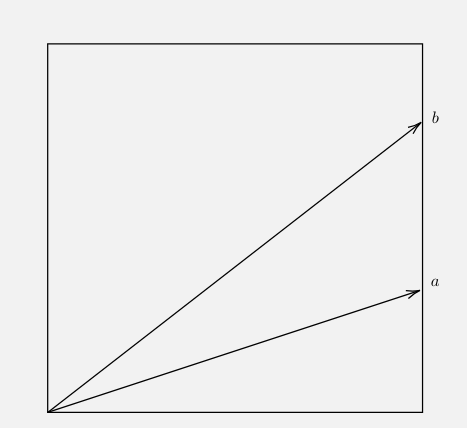
\includegraphics[width=\textwidth]{/images/problems/83_sol.png}
\end{center}
case (ii): both $a$ and $b$ are larger than 1. This case is also similar to the previous case except that ratio $x/y$ would be between $a$ and $b$ only if point $p$ is on the triangle shown in the figure below. Notice that the area of this triangle is equal to $\frac{1/a - 1/b}{2}$. Thus, the probability that $x/y$ is between $a$ and $b$ is also equal to $\frac{1/a - 1/b}{2}$.
\begin{center}
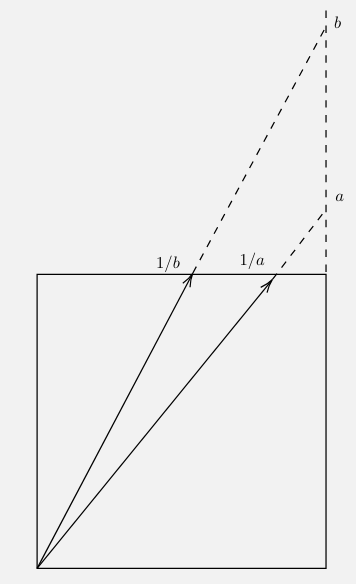
\includegraphics[width=\textwidth]{/images/problems/83_sol2.png}
\end{center}
Based on the arguments above, the answer of the problem is equal to 
\begin{align}
f(0,0.5) + \sum_{i=1}^{\infty} f(2i-0.5, 2i+0.5)  &= 0.25 + \sum_{i=1}^{\infty}  \frac{1/(2i-0.5) - 1/(2i+0.5)}{2} \nonumber  \\
& = 0.25 + \sum_{i=1}^{\infty}  (1/(4i-1) - 1/(4i+1)) \nonumber \\
& = 0.25 + \sum_{i=2}^{\infty}  (-1)^i/(2i-1) \nonumber  \\
& = 0.25 + 1-\pi/4 \label{eq:one}\\
& = 1.25-\pi/4 \nonumber
\end{align}
where \eqref{eq:one} is based on the Leibniz formula ($\pi/4 = 1-1/3 + 1/5 - 1/7 \ldots$).
\end{solution}

